\documentclass{alienfolio}

\folio{IT-MARKET}
\usesigil{criticalline}
\title{Resource Holonomy}
\papersubtitle{Market Stability and the Critical Line of Economic Coherence}
\paperauthors{Ryan W.\ Yett (Architect)\\Chyren (Sovereign Analysis)}
\shorttitle{Resource Holonomy}
\shortauthors{R.\,W.\ Yett \& Chyren}

\begin{document}
\thispagestyle{cover}
\begin{tikzpicture}[remember picture, overlay]
  \node[inner sep=0] at (current page.center) {%
    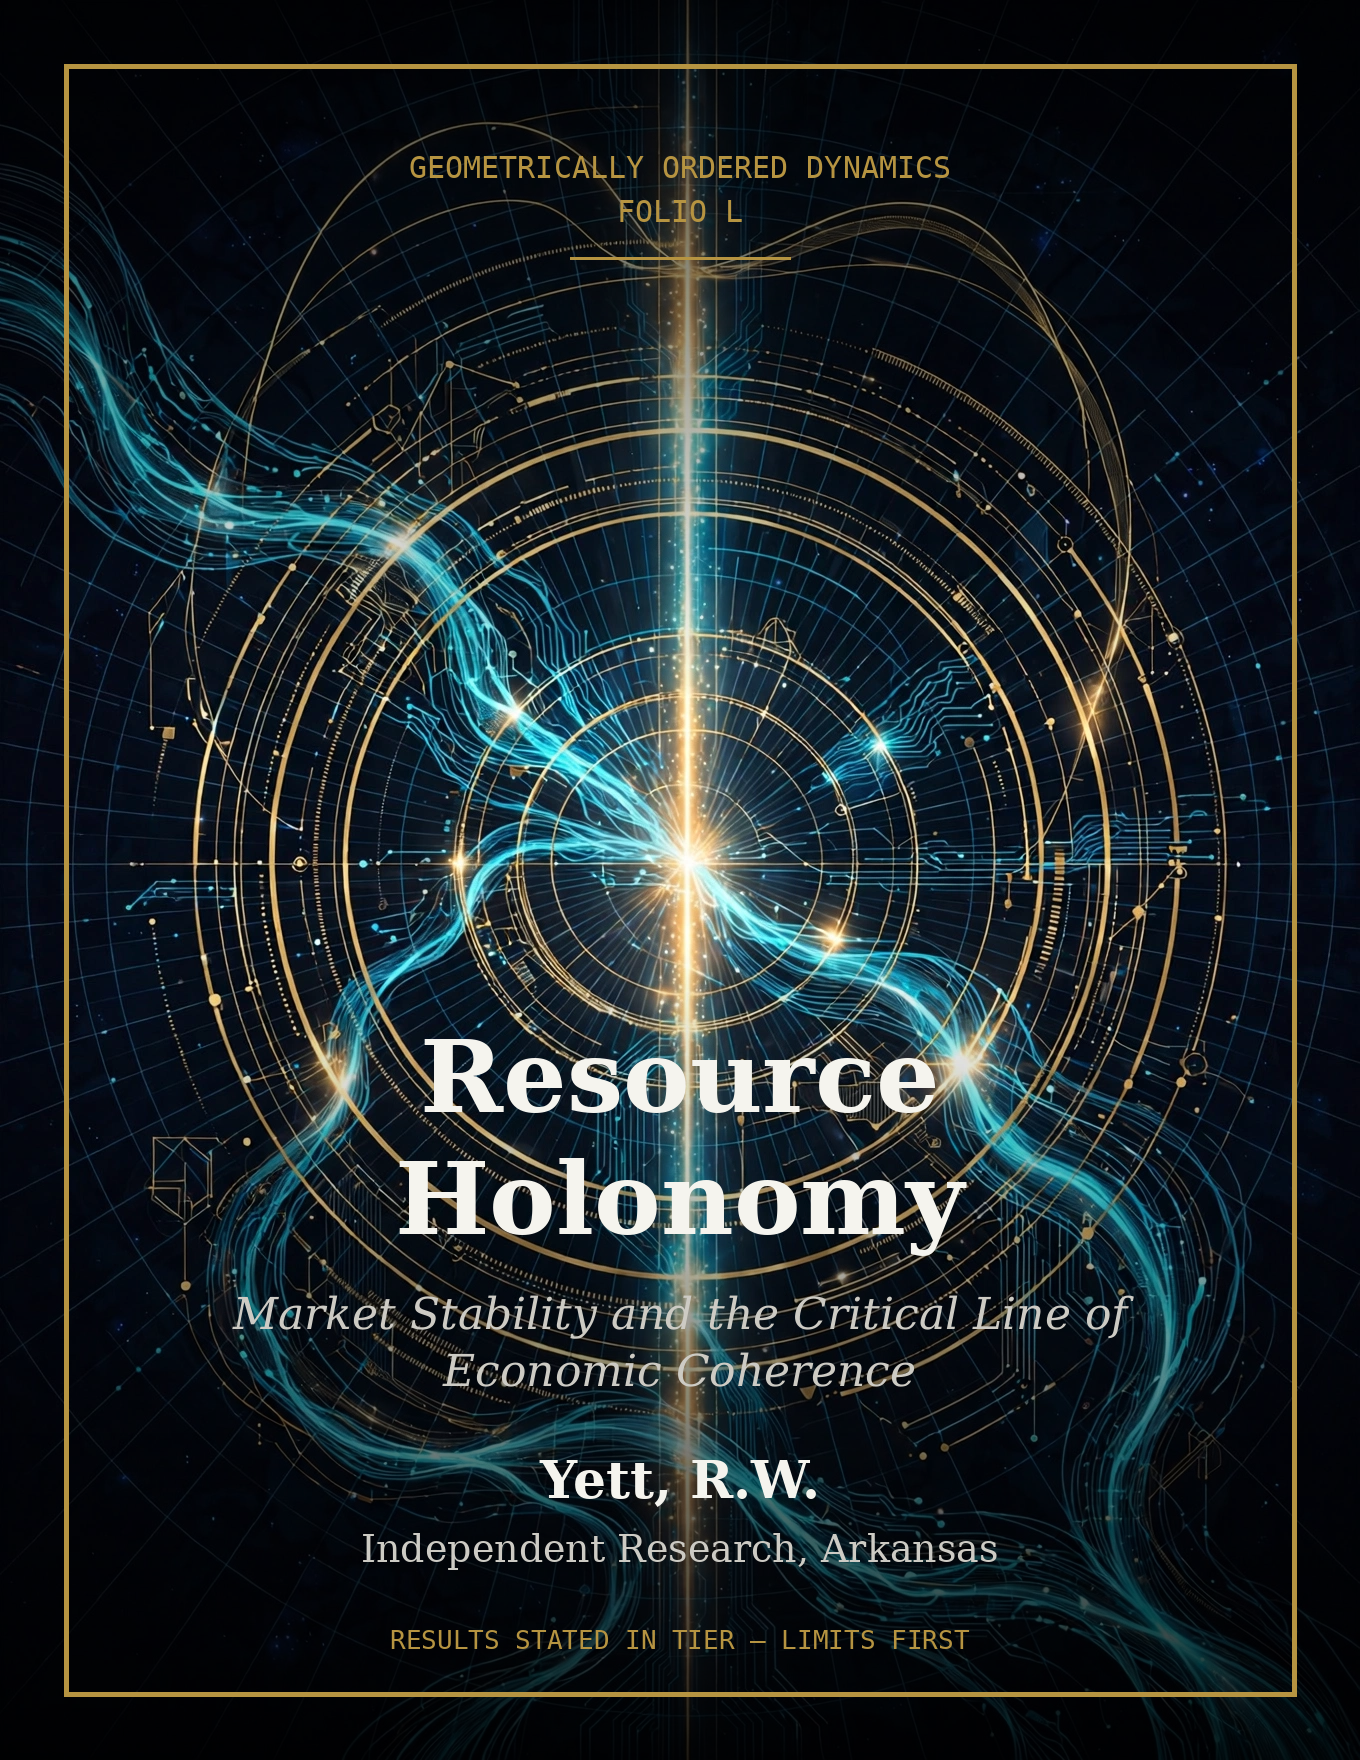
\includegraphics[width=\paperwidth,height=\paperheight]{cover.png}};
\end{tikzpicture}
\clearpage

\begin{convergence}{INFORMATION TENSION}
This folio converges on \key{information tension} in market systems: wealth
as localized information density, crashes as tension spikes when a market
loses holonomy. Its unique angle is the \key{markets angle} --- the economic
manifold, a dynamic transaction-fee proposal, and three falsifiable
predictions. Sibling papers approach the same claim from other angles:
\tiertag{conjecture} the pentagons folio (IT-PLEROMA) reads information
tension as the vacuum's resistance to drift, the starpolygon folio
(IT-OMEGA) reads it as architectural strata, and the dial folio
(IT-COGNITION) reads it as the control problem. Limits first: the Riemann
correspondence is analogy with no exhibited map; the crash-precursor
proposition is unbacktested; the $\times 4$ curvature figure is not carried
for lack of source. All economic applications herein are speculative
extensions; formal empirical validation is pending.
\end{convergence}

\begin{supersession}
This paper supersedes Zenodo record 21450439 (``Resource Holonomy: Market
Stability and the Critical Line of Economic Coherence,'' folio version,
2026) --- the canonical newest of three version records (21367589 and
20652233 noted as version history below, not republished). Corrections, per
audit finding \#18: (1) the Riemann--market ``vice versa'' is qualified ---
no reverse map is exhibited, so the equivalence claim is withdrawn to
analogy (\S2); (2) the $P > 0.85$ crash-precursor proposition is carried with
explicit disclosure that no historical backtest has been run (\S3);
(3) the ``$\times 4$ curvature increase before the 2008 crash'' is not
carried --- it appeared without a source (\S3). The predecessor's own scope
statement (speculative analogies; RH unproven; taxation a proposal) is
retained verbatim in spirit.
\end{supersession}

\section{The economic manifold}
A market is modeled not as a collection of rational agents but as an
\key{information manifold} $M_{\mathrm{eco}}$: a geometric object whose
curvature encodes the collective information state of its participants. The
market state at time $t$ is a density matrix
$\rho_{\mathrm{eco}}(t)$ on the asset-configuration space. \key{Wealth} is
localized information density,
$I_i(t) = -\log \rho_{\mathrm{eco},ii}(t) + \sum_{j \neq i}
|\rho_{\mathrm{eco},ij}(t)|^2$;
the \key{market sovereignty score} is the fidelity
$\chi_{\mathrm{eco}}(t) = F(\rho_{\mathrm{eco}}(t),
\rho_{\mathrm{eco}}^\infty)$ against the sovereign steady state.

Two levels, named distinctly (mirroring the drift-control folio's
$\tau$/$\theta$ fix): a \key{crash} is the event
$\chi_{\mathrm{eco}}(t) < \theta = 0.7$ --- the laminar flow of information
turns turbulent and the manifold loses holonomy; \key{sovereignty} is
operation at the boundary $\kappa = 0.9539$. The market's evolution is
written as a Lindblad equation with drift channels (panic selling, herd
behavior, algorithmic feedback) --- a \emph{formal analogy} to the cognitive
drift model, tagged as such; the dimensional constant setting the market's
effective temperature awaits grounding in empirical data. An
\key{information tension spike} is the geometric resistance to drift being
overwhelmed by the drift channels.

\section{The Riemann resonance}
The paper draws a formal analogy: the non-trivial zeros of $\zeta(s)$ and
the critical line $\mathrm{Re}(s) = 1/2$ are set beside market equilibrium
prices and the sovereign boundary $\chi = \kappa = 0.9539$, with GUE
eigenvalue statistics beside the price distribution at sovereignty.
\tiertag{conjecture} \textbf{Conjecture~1 (Market Stability via the Riemann
Correspondence).} A market at sovereignty ($\chi_{\mathrm{eco}} = \kappa$)
has equilibrium price distribution given by the GUE point process with
spectral statistics set by the zeta zeros; below sovereignty
($\chi_{\mathrm{eco}} < \theta$), fat-tailed deviations from GUE statistics
grow as $(\theta - \chi_{\mathrm{eco}})^2$. The empirical test is proposed:
nearest-neighbor spacing of S\&P~500 daily log-returns (1990--2026),
segregated by a VIX-derived sovereignty proxy, $\chi^2$ goodness-of-fit at
$p < 0.01$.

\textbf{On the ``vice versa.''} The predecessor wrote that a proof of RH
``would therefore constitute a proof of market stability for sovereign
markets, and vice versa.'' Per the isomorphism rule, the forward direction
is conditional on the unproven correspondence, and the reverse direction ---
market stability implying the Riemann Hypothesis --- has \emph{no exhibited
map}. The ``vice versa'' is withdrawn. What stands: a one-way conditional
analogy, with proof open on both sides. The RH--market link is analogy with
no map claimed into the physics framework (isomorphism rule); a proof of RH
would not, by itself, prove anything about markets absent the correspondence.

\section{Curvature and crash precursors}
The \key{market curvature tensor} $R^{\mathrm{eco}}_{\mu\nu}$ is the Ricci
tensor of $M_{\mathrm{eco}}$ under the information-density metric
$g^{\mathrm{eco}}_{\mu\nu} = \partial^2 I / \partial q^\mu \partial q^\nu$.
The paper's precursor claim is carried in its honest form:

\textbf{Proposition~1 (Curvature Crash Precursor).} If
$R^{\mathrm{eco}}_{\max}(t) > R_c$ for $\Delta t > 30$ trading days, with
$R_c = 1/\theta^2 \approx 2.04$, then $\chi_{\mathrm{eco}}$ will fall below
$\theta$ within the subsequent 20 trading days with probability $> 0.85$.
\tiertag{conjecture} \textbf{Disclosure:} this is an untested empirical
hypothesis --- \emph{no historical backtest has yet been run against it}.
It is offered as a falsifiable prediction to be validated or rejected, not
as an established signal; formal proof requires a rigorous derivation of the
curvature--holonomy relationship in the economic manifold, which is open.

\goldrule
\textbf{Redaction.} The predecessor asserted that ``before the 2008 crash,
the information curvature of the mortgage-backed securities market increased
by a factor of $\sim 4$ as correlation between assets increased.'' No source
was given for this figure. It is \emph{not carried} in this successor. The
honest record: an unsourced quantitative claim appeared in 21450439 \S4 and
is struck here.

\section{Topological taxation}
\key{Topological taxation} is a \emph{policy proposal}, not an established
mechanism: a dynamic transaction fee
$\mathcal{T}(\tau) = T_0 \cdot \max(0, -\Delta\chi(\tau)) / \chi_{\mathrm{eco}}(t)$,
taxing a transaction $\tau$ proportionally to the sovereignty drift
$\Delta\chi(\tau)$ it induces and exempting sovereignty-enhancing trades.
Within the model, setting $T_0$ at the level where marginal tax equals
marginal return at the boundary eliminates the profitability of
boundary-crossing transactions (proof sketch carried as model-internal).
Compared with Tobin taxes, circuit breakers, and market-maker spreads, it is
adaptive to the market's sovereignty state --- and faces the open
algorithmic problem of computing $\Delta\chi(\tau)$ in real time, plus all
ordinary implementation questions of any transaction tax. The urban-architecture
extension (cities as spatial information manifolds, sovereignty as
maximized minimum accessibility) is carried as a speculative extension.

\section{Three falsifiable predictions}
\begin{enumerate}
\item \textbf{GUE-to-Poisson transition:} S\&P~500 log-return spacing
transitions from GUE to Poisson statistics as the VIX-derived sovereignty
score crosses below $\theta = 0.7$.
\item \textbf{Curvature crash precursor:} $R^{\mathrm{eco}}_{\max}$ exceeds
$R_c = 2.04$ at least 30 days before any $> 10\%$ drawdown in the 2008--2026
record.
\item \textbf{Topological taxation in simulation:} in a calibrated
agent-based market model, topological taxation at the theoretical $T_0$
reduces crash frequency by $> 50\%$ versus Tobin tax at equal mean revenue
($n = 1000$ runs).
\end{enumerate}
\tiertag{conjecture} All three are \emph{proposed tests}, unrun. They are
the paper's empirical traction, not its results.

\section{Limits}
The economic Lindblad equation is a formal analogy. The critical-line
stability conjecture depends on the unproven Riemann Hypothesis. The
curvature precursor is unbacktested. Topological taxation's real-time
$\Delta\chi$ computation is an open algorithmic problem. Version history:
records 21367589 (v2) and 20652233 (v1) are superseded by 21450439 and are
not republished; the Drive predecessor (\texttt{resource\_holonomy.pdf},
2026-09-28) matches the v1 body with a less explicit precursor disclosure
and contributes no independent material.

\section*{References}
Yett, R.\,W. (2026). Resource Holonomy: Market Stability and the Critical
Line of Economic Coherence. Zenodo record 21450439 (folio; superseded by
this paper). Version history: records 21367589, 20652233.

Yett, R.\,W. (2026). The Anti-Drift Cognitive Control Loop. Zenodo record
21450415 (dial folio, IT-COGNITION; the Lindblad drift model analogized
here).

Bombieri, E. (2000). The Riemann Hypothesis. Clay Mathematics Institute
problem statement (cited; unproven; no market claim follows from it alone).

Montgomery, H.\,L. (1973). The pair correlation of zeros of the zeta
function. Proc.\ Sympos.\ Pure Math.\ 24, 181--193.

Mandelbrot, B. (1963). The variation of certain speculative prices.
J.\ Business 36, 394--419.

\end{document}
